\section{Simulator Class Reference}
\label{classSimulator}\index{Simulator@{Simulator}}
{\tt \#include $<$simulator.h$>$}

Collaboration diagram for Simulator:\nopagebreak
\begin{figure}[H]
\begin{center}
\leavevmode
\includegraphics[height=400pt]{classSimulator__coll__graph}
\end{center}
\end{figure}
\subsection*{Static Public Member Functions}
\begin{CompactItemize}
\item 
static void {\bf Run} ()
\item 
static void {\bf Stop} ()
\item 
static void {\bf StopAt} (double)
\item 
static double {\bf Now} ()
\item 
static bool {\bf Cancel} ({\bf EventId} \&)
\item 
static {\bf EventId} {\bf Peek} ()
\item 
static {\bf EventBase} $\ast$ {\bf GetEarliestEvent} ()
\item 
static int {\bf MyRank} ()
\item 
{\footnotesize template$<$typename T , typename OBJ $>$ }\\static {\bf EventId} {\bf Schedule} (double t, void(T::$\ast$handler)(void), OBJ $\ast$obj)
\item 
{\footnotesize template$<$typename T , typename OBJ , typename U1 , typename T1 $>$ }\\static {\bf EventId} {\bf Schedule} (double t, void(T::$\ast$handler)(U1), OBJ $\ast$obj, T1 t1)
\item 
{\footnotesize template$<$typename T , typename OBJ , typename U1 , typename T1 , typename U2 , typename T2 $>$ }\\static {\bf EventId} {\bf Schedule} (double t, void(T::$\ast$handler)(U1, U2), OBJ $\ast$obj, T1 t1, T2 t2)
\item 
{\footnotesize template$<$typename T , typename OBJ , typename U1 , typename T1 , typename U2 , typename T2 , typename U3 , typename T3 $>$ }\\static {\bf EventId} {\bf Schedule} (double t, void(T::$\ast$handler)(U1, U2, U3), OBJ $\ast$obj, T1 t1, T2 t2, T3 t3)
\item 
{\footnotesize template$<$typename T , typename OBJ , typename U1 , typename T1 , typename U2 , typename T2 , typename U3 , typename T3 , typename U4 , typename T4 $>$ }\\static {\bf EventId} {\bf Schedule} (double t, void(T::$\ast$handler)(U1, U2, U3, U4), OBJ $\ast$obj, T1 t1, T2 t2, T3 t3, T4 t4)
\item 
static {\bf EventId} {\bf Schedule} (double t, void($\ast$handler)(void))
\item 
{\footnotesize template$<$typename U1 , typename T1 $>$ }\\static {\bf EventId} {\bf Schedule} (double t, void($\ast$handler)(U1), T1 t1)
\item 
{\footnotesize template$<$typename U1 , typename T1 , typename U2 , typename T2 $>$ }\\static {\bf EventId} {\bf Schedule} (double t, void($\ast$handler)(U1, U2), T1 t1, T2 t2)
\item 
{\footnotesize template$<$typename U1 , typename T1 , typename U2 , typename T2 , typename U3 , typename T3 $>$ }\\static {\bf EventId} {\bf Schedule} (double t, void($\ast$handler)(U1, U2, U3), T1 t1, T2 t2, T3 t3)
\item 
{\footnotesize template$<$typename U1 , typename T1 , typename U2 , typename T2 , typename U3 , typename T3 , typename U4 , typename T4 $>$ }\\static {\bf EventId} {\bf Schedule} (double t, void($\ast$handler)(U1, U2, U3, U4), T1 t1, T2 t2, T3 t3, T4 t4)
\item 
static void {\bf registerComponent} ({\bf Component} $\ast$obj, int lp)
\item 
static {\bf ComponentDescription} $\ast$ {\bf getComponentDesc} (int)
\end{CompactItemize}
\subsection*{Static Private Attributes}
\begin{CompactItemize}
\item 
static {\bf EventSet\_\-t} {\bf events}
\item 
static double {\bf simTime}
\item 
static {\bf ComponentMap\_\-t} {\bf components}
\item 
static int {\bf nextComponentID}
\item 
static int {\bf rank}
\item 
static bool {\bf halted} = false
\end{CompactItemize}


\subsection{Detailed Description}


Definition at line 296 of file simulator.h.

\subsection{Member Function Documentation}
\index{Simulator@{Simulator}!Cancel@{Cancel}}
\index{Cancel@{Cancel}!Simulator@{Simulator}}
\subsubsection[{Cancel}]{\setlength{\rightskip}{0pt plus 5cm}bool Simulator::Cancel ({\bf EventId} \& {\em evid})\hspace{0.3cm}{\tt  [static]}}\label{classSimulator_f85320c35a3ef59e17244e53047a4501}




Definition at line 56 of file simulator.cc.

References events.\index{Simulator@{Simulator}!getComponentDesc@{getComponentDesc}}
\index{getComponentDesc@{getComponentDesc}!Simulator@{Simulator}}
\subsubsection[{getComponentDesc}]{\setlength{\rightskip}{0pt plus 5cm}{\bf ComponentDescription} $\ast$ Simulator::getComponentDesc (int {\em compId})\hspace{0.3cm}{\tt  [static]}}\label{classSimulator_664a4bdb8925e0251e94131192743ff2}




Definition at line 101 of file simulator.cc.

References components.

Referenced by Link::Link(), and Link::Send().

Here is the caller graph for this function:\nopagebreak
\begin{figure}[H]
\begin{center}
\leavevmode
\includegraphics[width=147pt]{classSimulator_664a4bdb8925e0251e94131192743ff2_icgraph}
\end{center}
\end{figure}
\index{Simulator@{Simulator}!GetEarliestEvent@{GetEarliestEvent}}
\index{GetEarliestEvent@{GetEarliestEvent}!Simulator@{Simulator}}
\subsubsection[{GetEarliestEvent}]{\setlength{\rightskip}{0pt plus 5cm}{\bf EventBase} $\ast$ Simulator::GetEarliestEvent ()\hspace{0.3cm}{\tt  [static]}}\label{classSimulator_766aee01e48e500f84af435626ab7004}




Definition at line 71 of file simulator.cc.

References events.\index{Simulator@{Simulator}!MyRank@{MyRank}}
\index{MyRank@{MyRank}!Simulator@{Simulator}}
\subsubsection[{MyRank}]{\setlength{\rightskip}{0pt plus 5cm}int Simulator::MyRank ()\hspace{0.3cm}{\tt  [static]}}\label{classSimulator_80bffbd51839958866ddd16fde614ecf}




Definition at line 78 of file simulator.cc.

References rank.

Referenced by Link::Link(), and Link::Send().

Here is the caller graph for this function:\nopagebreak
\begin{figure}[H]
\begin{center}
\leavevmode
\includegraphics[width=122pt]{classSimulator_80bffbd51839958866ddd16fde614ecf_icgraph}
\end{center}
\end{figure}
\index{Simulator@{Simulator}!Now@{Now}}
\index{Now@{Now}!Simulator@{Simulator}}
\subsubsection[{Now}]{\setlength{\rightskip}{0pt plus 5cm}double Simulator::Now ()\hspace{0.3cm}{\tt  [static]}}\label{classSimulator_cf5727f517db6743ddf25ae7cc9a8db4}




Definition at line 51 of file simulator.cc.

References simTime.

Referenced by CmdIssuer::BankNotBusy(), CmdIssuer::BusNotBusy(), Statistic::CalculateAggregateStats(), CmdIssuer::CanSchedule(), Clock::Clock(), Statistic::CollectStatsPerRequest(), MSHR\_\-SA\_\-H::DeleteInMSHR(), MSHR\_\-H::DeleteInMSHR(), MSHR\_\-SA\_\-H::demap\_\-addr(), MSHR\_\-H::demap\_\-addr(), PToPSwitchArbiter::do\_\-fcfs\_\-arbitration(), PToPSwitchArbiterVcs::do\_\-round\_\-robin\_\-arbitration(), GenericRouterVct::do\_\-switch\_\-traversal(), GenericRouterVcs::do\_\-switch\_\-traversal(), GenericRouterNoVcs::do\_\-switch\_\-traversal(), GenericRouterAdaptive::do\_\-switch\_\-traversal(), uncore\_\-t::enqueue(), Clock::fallingEdge(), GenericTPGVcs::GetNewRequest(), GenericTPG::GetNewRequest(), GenericRouterVcs::handle\_\-detect\_\-deadlock\_\-event(), GenericInterfaceVcs::handle\_\-link\_\-arrival(), GenericInterface::handle\_\-link\_\-arrival(), GenericRouterVct::handle\_\-link\_\-arrival\_\-event(), GenericRouterVcs::handle\_\-link\_\-arrival\_\-event(), GenericRouterNoVcs::handle\_\-link\_\-arrival\_\-event(), GenericLink::handle\_\-link\_\-arrival\_\-event(), GenericRouterAdaptive::handle\_\-link\_\-arrival\_\-event\_\-multiple\_\-flit\_\-in\_\-buffer(), GenericRouterAdaptive::handle\_\-link\_\-arrival\_\-event\_\-one\_\-msg\_\-per\_\-buffer(), uncore\_\-t::handle\_\-new\_\-packet\_\-event(), NI::handle\_\-new\_\-packet\_\-event(), GenericTPGVcs::handle\_\-new\_\-packet\_\-event(), GenericTPG::handle\_\-new\_\-packet\_\-event(), GenericSink::handle\_\-new\_\-packet\_\-event(), GenericRPG::handle\_\-new\_\-packet\_\-event(), GenericInterfaceVcs::handle\_\-new\_\-packet\_\-event(), GenericInterface::handle\_\-new\_\-packet\_\-event(), GenericFlatMc::handle\_\-new\_\-packet\_\-event(), NI::handle\_\-out\_\-pull\_\-event(), GenericTPGVcs::handle\_\-out\_\-pull\_\-event(), GenericTPG::handle\_\-out\_\-pull\_\-event(), GenericRPG::handle\_\-out\_\-pull\_\-event(), GenericFlatMc::handle\_\-out\_\-pull\_\-event(), GenericSink::handle\_\-outpull\_\-event(), NI::handle\_\-ready\_\-event(), GenericTPGVcs::handle\_\-ready\_\-event(), GenericTPG::handle\_\-ready\_\-event(), GenericSink::handle\_\-ready\_\-event(), GenericRPG::handle\_\-ready\_\-event(), GenericInterfaceVcs::handle\_\-ready\_\-event(), GenericInterface::handle\_\-ready\_\-event(), GenericFlatMc::handle\_\-ready\_\-event(), GenericRouterVct::handle\_\-tick\_\-event(), GenericRouterVcs::handle\_\-tick\_\-event(), GenericRouterNoVcs::handle\_\-tick\_\-event(), GenericRouterAdaptive::handle\_\-tick\_\-event(), GenericInterfaceVcs::handle\_\-tick\_\-event(), GenericInterface::handle\_\-tick\_\-event(), HighLevelPacket::HighLevelPacket(), GenericRouterVcs::init(), GenericRouterAdaptive::init\_\-buffer\_\-state(), main(), Statistic::PrintAggregateStats(), ResponseHandler::process\_\-event(), RequestHandler::process\_\-event(), RefreshMgr::process\_\-event(), MSHR\_\-SA\_\-H::process\_\-event(), MSHR\_\-H::process\_\-event(), DRAMChannel::process\_\-event(), DataBusHandler::process\_\-event(), CmdIssuer::process\_\-event(), CmdBusHandler::process\_\-event(), BankHandler::process\_\-event(), AddrMap::process\_\-event(), PToPSwitchArbiterVcs::request(), PToPSwitchArbiter::request(), Clock::risingEdge(), Link::Send(), GenericRouterVct::send\_\-credit\_\-back(), GenericRouterVcs::send\_\-credit\_\-back(), GenericRouterNoVcs::send\_\-credit\_\-back(), GenericRouterAdaptive::send\_\-credit\_\-back(), CmdIssuer::SetBusBusyTime(), CmdIssuer::SetPrevState(), GenericTPGVcs::setup(), GenericTPG::setup(), GenericSink::setup(), GenericRPG::setup(), GenericFlatMc::setup(), MC::sim\_\-main(), MC::StartRefresh(), TailFlit::TailFlit(), and IrisEvent::toString().\index{Simulator@{Simulator}!Peek@{Peek}}
\index{Peek@{Peek}!Simulator@{Simulator}}
\subsubsection[{Peek}]{\setlength{\rightskip}{0pt plus 5cm}{\bf EventId} Simulator::Peek ()\hspace{0.3cm}{\tt  [static]}}\label{classSimulator_b70ac4a1b36c3a20e7548203d22b9c17}




Definition at line 64 of file simulator.cc.

References events.\index{Simulator@{Simulator}!registerComponent@{registerComponent}}
\index{registerComponent@{registerComponent}!Simulator@{Simulator}}
\subsubsection[{registerComponent}]{\setlength{\rightskip}{0pt plus 5cm}void Simulator::registerComponent ({\bf Component} $\ast$ {\em obj}, \/  int {\em lp})\hspace{0.3cm}{\tt  [static]}}\label{classSimulator_bc27a87849e9903771b3990c99c750bd}




Definition at line 85 of file simulator.cc.

References components, nextComponentID, rank, and Component::setComponentId().

Referenced by Component::Component().

Here is the caller graph for this function:\nopagebreak
\begin{figure}[H]
\begin{center}
\leavevmode
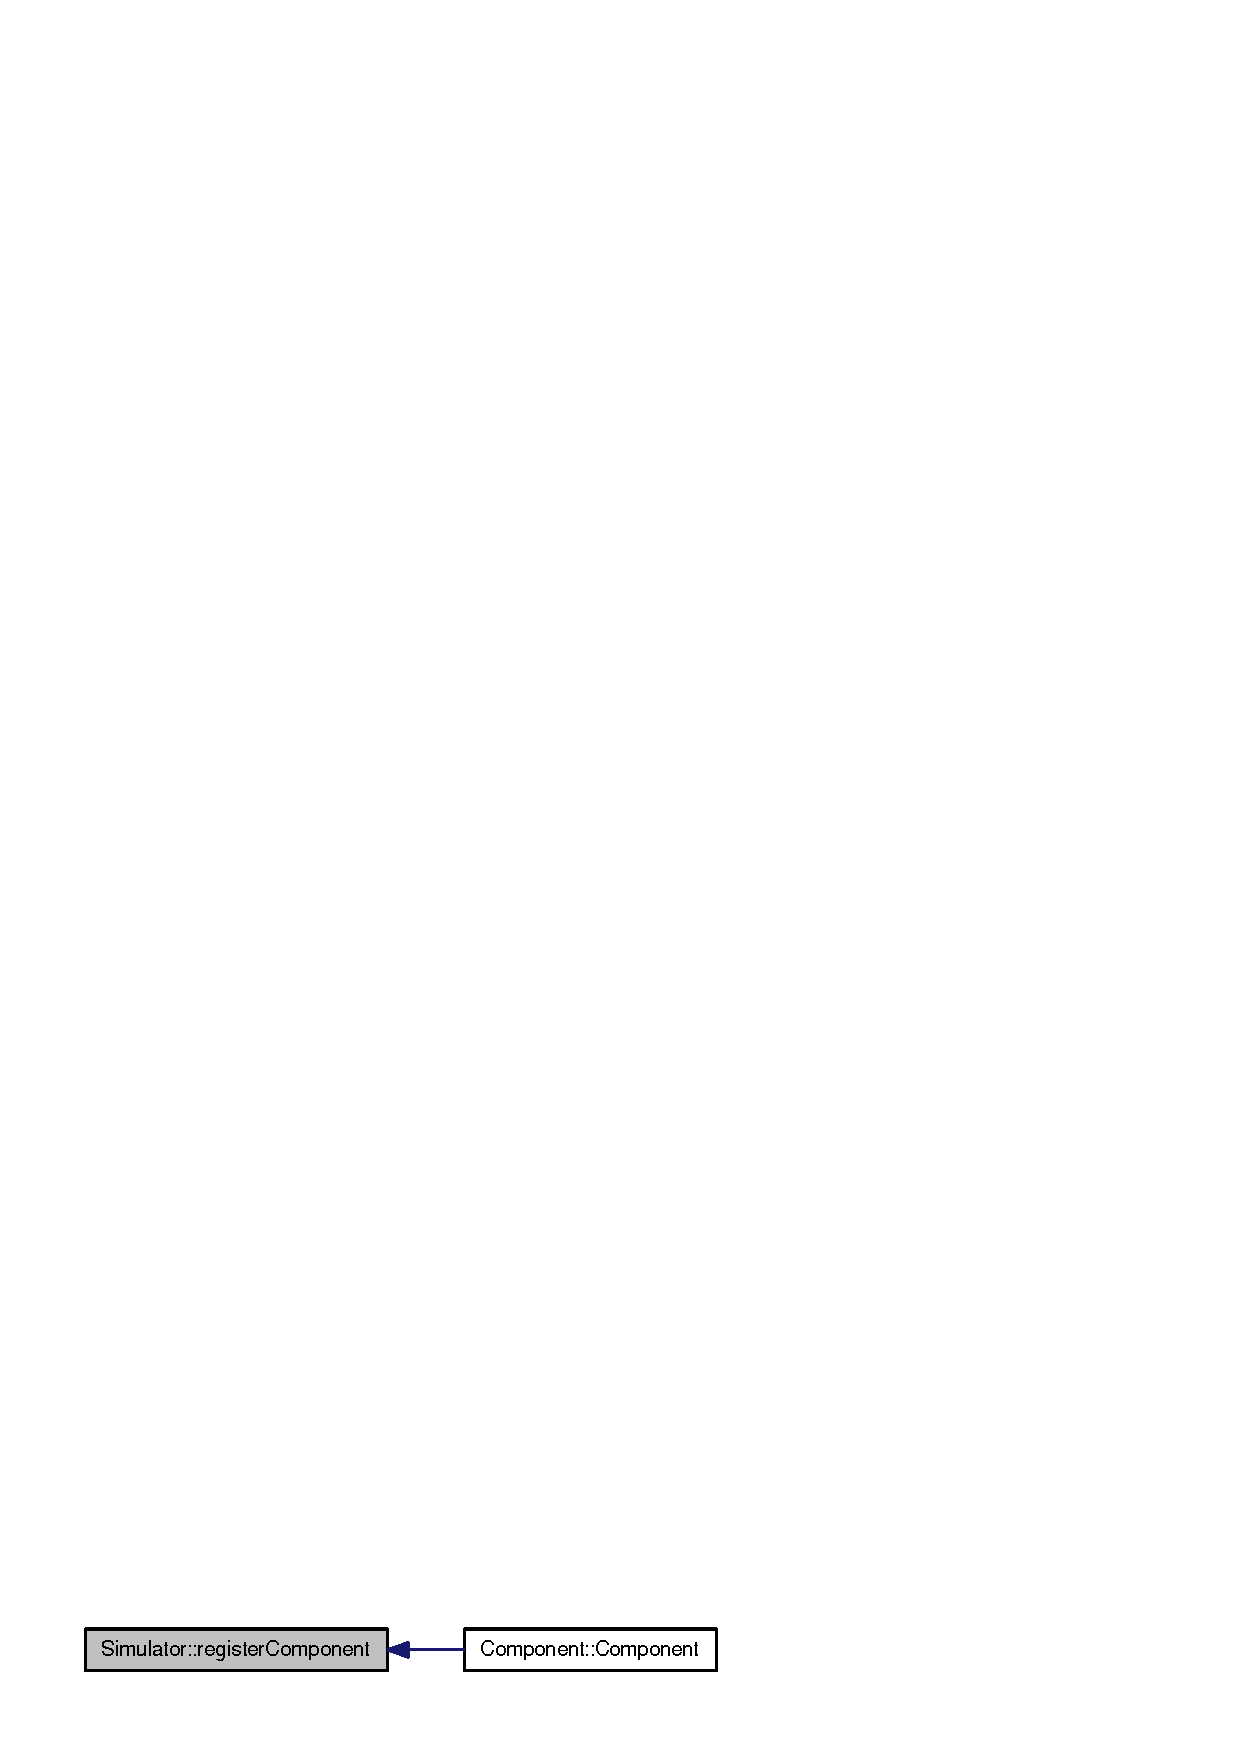
\includegraphics[width=174pt]{classSimulator_bc27a87849e9903771b3990c99c750bd_icgraph}
\end{center}
\end{figure}
\index{Simulator@{Simulator}!Run@{Run}}
\index{Run@{Run}!Simulator@{Simulator}}
\subsubsection[{Run}]{\setlength{\rightskip}{0pt plus 5cm}void Simulator::Run ()\hspace{0.3cm}{\tt  [static]}}\label{classSimulator_27e7045e7aa4e29e9d2003aaa09c8326}




Definition at line 21 of file simulator.cc.

References EventBase::CallHandler(), events, halted, rank, simTime, and EventBase::time.

Referenced by main().

Here is the caller graph for this function:\nopagebreak
\begin{figure}[H]
\begin{center}
\leavevmode
\includegraphics[width=100pt]{classSimulator_27e7045e7aa4e29e9d2003aaa09c8326_icgraph}
\end{center}
\end{figure}
\index{Simulator@{Simulator}!Schedule@{Schedule}}
\index{Schedule@{Schedule}!Simulator@{Simulator}}
\subsubsection[{Schedule}]{\setlength{\rightskip}{0pt plus 5cm}template$<$typename U1 , typename T1 , typename U2 , typename T2 , typename U3 , typename T3 , typename U4 , typename T4 $>$ static {\bf EventId} Simulator::Schedule (double {\em t}, \/  void($\ast$)(U1, U2, U3, U4) {\em handler}, \/  T1 {\em t1}, \/  T2 {\em t2}, \/  T3 {\em t3}, \/  T4 {\em t4})\hspace{0.3cm}{\tt  [inline, static]}}\label{classSimulator_a94a8a5c64b661ad4607517d84c8832e}




Definition at line 397 of file simulator.h.

References events, and EventBase::uid.\index{Simulator@{Simulator}!Schedule@{Schedule}}
\index{Schedule@{Schedule}!Simulator@{Simulator}}
\subsubsection[{Schedule}]{\setlength{\rightskip}{0pt plus 5cm}template$<$typename U1 , typename T1 , typename U2 , typename T2 , typename U3 , typename T3 $>$ static {\bf EventId} Simulator::Schedule (double {\em t}, \/  void($\ast$)(U1, U2, U3) {\em handler}, \/  T1 {\em t1}, \/  T2 {\em t2}, \/  T3 {\em t3})\hspace{0.3cm}{\tt  [inline, static]}}\label{classSimulator_2bc6f517e3b3a284b6b52efc47a9da76}




Definition at line 386 of file simulator.h.

References events, and EventBase::uid.\index{Simulator@{Simulator}!Schedule@{Schedule}}
\index{Schedule@{Schedule}!Simulator@{Simulator}}
\subsubsection[{Schedule}]{\setlength{\rightskip}{0pt plus 5cm}template$<$typename U1 , typename T1 , typename U2 , typename T2 $>$ static {\bf EventId} Simulator::Schedule (double {\em t}, \/  void($\ast$)(U1, U2) {\em handler}, \/  T1 {\em t1}, \/  T2 {\em t2})\hspace{0.3cm}{\tt  [inline, static]}}\label{classSimulator_612e0d3f87f3461aa116ca3552adf11a}




Definition at line 376 of file simulator.h.

References events, and EventBase::uid.\index{Simulator@{Simulator}!Schedule@{Schedule}}
\index{Schedule@{Schedule}!Simulator@{Simulator}}
\subsubsection[{Schedule}]{\setlength{\rightskip}{0pt plus 5cm}template$<$typename U1 , typename T1 $>$ static {\bf EventId} Simulator::Schedule (double {\em t}, \/  void($\ast$)(U1) {\em handler}, \/  T1 {\em t1})\hspace{0.3cm}{\tt  [inline, static]}}\label{classSimulator_e76c104f5cfd844df6054a3c7956a098}




Definition at line 367 of file simulator.h.

References events, and EventBase::uid.\index{Simulator@{Simulator}!Schedule@{Schedule}}
\index{Schedule@{Schedule}!Simulator@{Simulator}}
\subsubsection[{Schedule}]{\setlength{\rightskip}{0pt plus 5cm}static {\bf EventId} Simulator::Schedule (double {\em t}, \/  void($\ast$)(void) {\em handler})\hspace{0.3cm}{\tt  [inline, static]}}\label{classSimulator_e5e8a4479b8e2a7b4ecdb3eb8561b960}




Definition at line 359 of file simulator.h.

References events, and EventBase::uid.\index{Simulator@{Simulator}!Schedule@{Schedule}}
\index{Schedule@{Schedule}!Simulator@{Simulator}}
\subsubsection[{Schedule}]{\setlength{\rightskip}{0pt plus 5cm}template$<$typename T , typename OBJ , typename U1 , typename T1 , typename U2 , typename T2 , typename U3 , typename T3 , typename U4 , typename T4 $>$ static {\bf EventId} Simulator::Schedule (double {\em t}, \/  void(T::$\ast$)(U1, U2, U3, U4) {\em handler}, \/  OBJ $\ast$ {\em obj}, \/  T1 {\em t1}, \/  T2 {\em t2}, \/  T3 {\em t3}, \/  T4 {\em t4})\hspace{0.3cm}{\tt  [inline, static]}}\label{classSimulator_6846b3f0aa16ad7b4a4a1653837c123a}




Definition at line 351 of file simulator.h.

References events, and EventBase::uid.\index{Simulator@{Simulator}!Schedule@{Schedule}}
\index{Schedule@{Schedule}!Simulator@{Simulator}}
\subsubsection[{Schedule}]{\setlength{\rightskip}{0pt plus 5cm}template$<$typename T , typename OBJ , typename U1 , typename T1 , typename U2 , typename T2 , typename U3 , typename T3 $>$ static {\bf EventId} Simulator::Schedule (double {\em t}, \/  void(T::$\ast$)(U1, U2, U3) {\em handler}, \/  OBJ $\ast$ {\em obj}, \/  T1 {\em t1}, \/  T2 {\em t2}, \/  T3 {\em t3})\hspace{0.3cm}{\tt  [inline, static]}}\label{classSimulator_f4102ccb431eea8143497cb92fb499d4}




Definition at line 339 of file simulator.h.

References events, and EventBase::uid.\index{Simulator@{Simulator}!Schedule@{Schedule}}
\index{Schedule@{Schedule}!Simulator@{Simulator}}
\subsubsection[{Schedule}]{\setlength{\rightskip}{0pt plus 5cm}template$<$typename T , typename OBJ , typename U1 , typename T1 , typename U2 , typename T2 $>$ static {\bf EventId} Simulator::Schedule (double {\em t}, \/  void(T::$\ast$)(U1, U2) {\em handler}, \/  OBJ $\ast$ {\em obj}, \/  T1 {\em t1}, \/  T2 {\em t2})\hspace{0.3cm}{\tt  [inline, static]}}\label{classSimulator_bb9b661fcd4fcbb62c331ef07a53eb7d}




Definition at line 328 of file simulator.h.

References events, and EventBase::uid.\index{Simulator@{Simulator}!Schedule@{Schedule}}
\index{Schedule@{Schedule}!Simulator@{Simulator}}
\subsubsection[{Schedule}]{\setlength{\rightskip}{0pt plus 5cm}template$<$typename T , typename OBJ , typename U1 , typename T1 $>$ static {\bf EventId} Simulator::Schedule (double {\em t}, \/  void(T::$\ast$)(U1) {\em handler}, \/  OBJ $\ast$ {\em obj}, \/  T1 {\em t1})\hspace{0.3cm}{\tt  [inline, static]}}\label{classSimulator_f483426f923de97d0f71ff88beceedbe}




Definition at line 318 of file simulator.h.

References events, and EventBase::uid.\index{Simulator@{Simulator}!Schedule@{Schedule}}
\index{Schedule@{Schedule}!Simulator@{Simulator}}
\subsubsection[{Schedule}]{\setlength{\rightskip}{0pt plus 5cm}template$<$typename T , typename OBJ $>$ static {\bf EventId} Simulator::Schedule (double {\em t}, \/  void(T::$\ast$)(void) {\em handler}, \/  OBJ $\ast$ {\em obj})\hspace{0.3cm}{\tt  [inline, static]}}\label{classSimulator_2b4be0a76ed9915d4c1c861386d666bc}




Definition at line 309 of file simulator.h.

References events, and EventBase::uid.

Referenced by Clock::Clock(), GenericRouterVct::do\_\-switch\_\-traversal(), GenericRouterVcs::do\_\-switch\_\-traversal(), GenericRouterNoVcs::do\_\-switch\_\-traversal(), GenericRouterAdaptive::do\_\-switch\_\-traversal(), uncore\_\-t::enqueue(), Clock::fallingEdge(), GenericRouterVcs::handle\_\-detect\_\-deadlock\_\-event(), GenericInterfaceVcs::handle\_\-link\_\-arrival(), GenericInterface::handle\_\-link\_\-arrival(), GenericRouterVct::handle\_\-link\_\-arrival\_\-event(), GenericRouterVcs::handle\_\-link\_\-arrival\_\-event(), GenericRouterNoVcs::handle\_\-link\_\-arrival\_\-event(), GenericLink::handle\_\-link\_\-arrival\_\-event(), GenericRouterAdaptive::handle\_\-link\_\-arrival\_\-event\_\-multiple\_\-flit\_\-in\_\-buffer(), GenericRouterAdaptive::handle\_\-link\_\-arrival\_\-event\_\-one\_\-msg\_\-per\_\-buffer(), uncore\_\-t::handle\_\-new\_\-packet\_\-event(), NI::handle\_\-new\_\-packet\_\-event(), GenericTPGVcs::handle\_\-new\_\-packet\_\-event(), GenericTPG::handle\_\-new\_\-packet\_\-event(), GenericSink::handle\_\-new\_\-packet\_\-event(), GenericRPG::handle\_\-new\_\-packet\_\-event(), GenericInterfaceVcs::handle\_\-new\_\-packet\_\-event(), GenericInterface::handle\_\-new\_\-packet\_\-event(), GenericFlatMc::handle\_\-new\_\-packet\_\-event(), NI::handle\_\-out\_\-pull\_\-event(), GenericTPGVcs::handle\_\-out\_\-pull\_\-event(), GenericTPG::handle\_\-out\_\-pull\_\-event(), GenericRPG::handle\_\-out\_\-pull\_\-event(), GenericFlatMc::handle\_\-out\_\-pull\_\-event(), GenericSink::handle\_\-outpull\_\-event(), NI::handle\_\-ready\_\-event(), GenericTPGVcs::handle\_\-ready\_\-event(), GenericTPG::handle\_\-ready\_\-event(), GenericSink::handle\_\-ready\_\-event(), GenericRPG::handle\_\-ready\_\-event(), GenericInterfaceVcs::handle\_\-ready\_\-event(), GenericInterface::handle\_\-ready\_\-event(), GenericFlatMc::handle\_\-ready\_\-event(), GenericRouterVct::handle\_\-tick\_\-event(), GenericRouterVcs::handle\_\-tick\_\-event(), GenericRouterNoVcs::handle\_\-tick\_\-event(), GenericRouterAdaptive::handle\_\-tick\_\-event(), GenericInterfaceVcs::handle\_\-tick\_\-event(), GenericInterface::handle\_\-tick\_\-event(), GenericRouterVcs::init(), main(), ResponseHandler::process\_\-event(), RequestHandler::process\_\-event(), RefreshMgr::process\_\-event(), MSHR\_\-SA\_\-H::process\_\-event(), MSHR\_\-H::process\_\-event(), DRAMChannel::process\_\-event(), DataBusHandler::process\_\-event(), CmdIssuer::process\_\-event(), CmdBusHandler::process\_\-event(), BankHandler::process\_\-event(), AddrMap::process\_\-event(), Clock::risingEdge(), Link::Send(), GenericRouterVct::send\_\-credit\_\-back(), GenericRouterVcs::send\_\-credit\_\-back(), GenericRouterNoVcs::send\_\-credit\_\-back(), GenericRouterAdaptive::send\_\-credit\_\-back(), GenericTPGVcs::setup(), GenericTPG::setup(), GenericSink::setup(), GenericRPG::setup(), GenericFlatMc::setup(), MC::sim\_\-main(), MC::StartRefresh(), and StopAt().\index{Simulator@{Simulator}!Stop@{Stop}}
\index{Stop@{Stop}!Simulator@{Simulator}}
\subsubsection[{Stop}]{\setlength{\rightskip}{0pt plus 5cm}void Simulator::Stop ()\hspace{0.3cm}{\tt  [static]}}\label{classSimulator_d493423e80256f53c715bb59c16ec78e}




Definition at line 41 of file simulator.cc.

References halted.

Referenced by StopAt().

Here is the caller graph for this function:\nopagebreak
\begin{figure}[H]
\begin{center}
\leavevmode
\includegraphics[width=166pt]{classSimulator_d493423e80256f53c715bb59c16ec78e_icgraph}
\end{center}
\end{figure}
\index{Simulator@{Simulator}!StopAt@{StopAt}}
\index{StopAt@{StopAt}!Simulator@{Simulator}}
\subsubsection[{StopAt}]{\setlength{\rightskip}{0pt plus 5cm}void Simulator::StopAt (double {\em stopTime})\hspace{0.3cm}{\tt  [static]}}\label{classSimulator_5611e1169517890edfeeb33f91281dd8}




Definition at line 46 of file simulator.cc.

References Schedule(), and Stop().

Referenced by main().

Here is the caller graph for this function:\nopagebreak
\begin{figure}[H]
\begin{center}
\leavevmode
\includegraphics[width=106pt]{classSimulator_5611e1169517890edfeeb33f91281dd8_icgraph}
\end{center}
\end{figure}


\subsection{Member Data Documentation}
\index{Simulator@{Simulator}!components@{components}}
\index{components@{components}!Simulator@{Simulator}}
\subsubsection[{components}]{\setlength{\rightskip}{0pt plus 5cm}{\bf ComponentMap\_\-t} {\bf Simulator::components}\hspace{0.3cm}{\tt  [static, private]}}\label{classSimulator_43a4085bf6efd14a954a2a078d2d8f19}




Definition at line 410 of file simulator.h.

Referenced by getComponentDesc(), and registerComponent().\index{Simulator@{Simulator}!events@{events}}
\index{events@{events}!Simulator@{Simulator}}
\subsubsection[{events}]{\setlength{\rightskip}{0pt plus 5cm}{\bf EventSet\_\-t} {\bf Simulator::events}\hspace{0.3cm}{\tt  [static, private]}}\label{classSimulator_4dc17b94fbab63fe9a7f44c9addf0df3}




Definition at line 408 of file simulator.h.

Referenced by Cancel(), GetEarliestEvent(), Peek(), Run(), and Schedule().\index{Simulator@{Simulator}!halted@{halted}}
\index{halted@{halted}!Simulator@{Simulator}}
\subsubsection[{halted}]{\setlength{\rightskip}{0pt plus 5cm}bool {\bf Simulator::halted} = false\hspace{0.3cm}{\tt  [static, private]}}\label{classSimulator_2fbf0fb13aebc2ba3e2b4a1140a5f92a}




Definition at line 413 of file simulator.h.

Referenced by main(), Run(), and Stop().\index{Simulator@{Simulator}!nextComponentID@{nextComponentID}}
\index{nextComponentID@{nextComponentID}!Simulator@{Simulator}}
\subsubsection[{nextComponentID}]{\setlength{\rightskip}{0pt plus 5cm}int {\bf Simulator::nextComponentID}\hspace{0.3cm}{\tt  [static, private]}}\label{classSimulator_c6b0293986cf31600e16177d0f29d3f9}




Definition at line 411 of file simulator.h.

Referenced by registerComponent().\index{Simulator@{Simulator}!rank@{rank}}
\index{rank@{rank}!Simulator@{Simulator}}
\subsubsection[{rank}]{\setlength{\rightskip}{0pt plus 5cm}int {\bf Simulator::rank}\hspace{0.3cm}{\tt  [static, private]}}\label{classSimulator_c4c86b1cdd6fb0032c0c2f8ee6babc34}




Definition at line 412 of file simulator.h.

Referenced by MyRank(), registerComponent(), and Run().\index{Simulator@{Simulator}!simTime@{simTime}}
\index{simTime@{simTime}!Simulator@{Simulator}}
\subsubsection[{simTime}]{\setlength{\rightskip}{0pt plus 5cm}double {\bf Simulator::simTime}\hspace{0.3cm}{\tt  [static, private]}}\label{classSimulator_a614fd7f680e5577786795d7ae3c077e}




Definition at line 409 of file simulator.h.

Referenced by Now(), and Run().

The documentation for this class was generated from the following files:\begin{CompactItemize}
\item 
{\bf simulator.h}\item 
{\bf simulator.cc}\end{CompactItemize}
